\section{Repairing Strategy : Constraint Automata}
\label{sec:strgCA}

\subsection{General Structure}
\label{subsec:generalCA}

\emph{Constraint automata} is a formalism to describe the behavior and possible
data flow in coordination models. 
Mostly used for model checking. We have used it for the purpose of program
repairing technique. Here we define the finite state automata as follows :

$$(Q, \Sigma, \delta, q_0, F)$$
\begin{itemize}
	\item $Q$: set of state where $|Q| = 2$, \emph{legal state}(init) and
\emph{illegal state} (error).
	\item $\Sigma$: symbols, invariants based on exception type.
	\item $\delta$: transition function. $init \rightarrow init$ is safe
transition and $init \rightarrow error$ is the invariant violation.
	\item $q_0$: starting state, here $q_0 = init$.
	\item $F$: end state, here it same as $q_0$.
\end{itemize}

\begin{figure}[!htb]
\centering
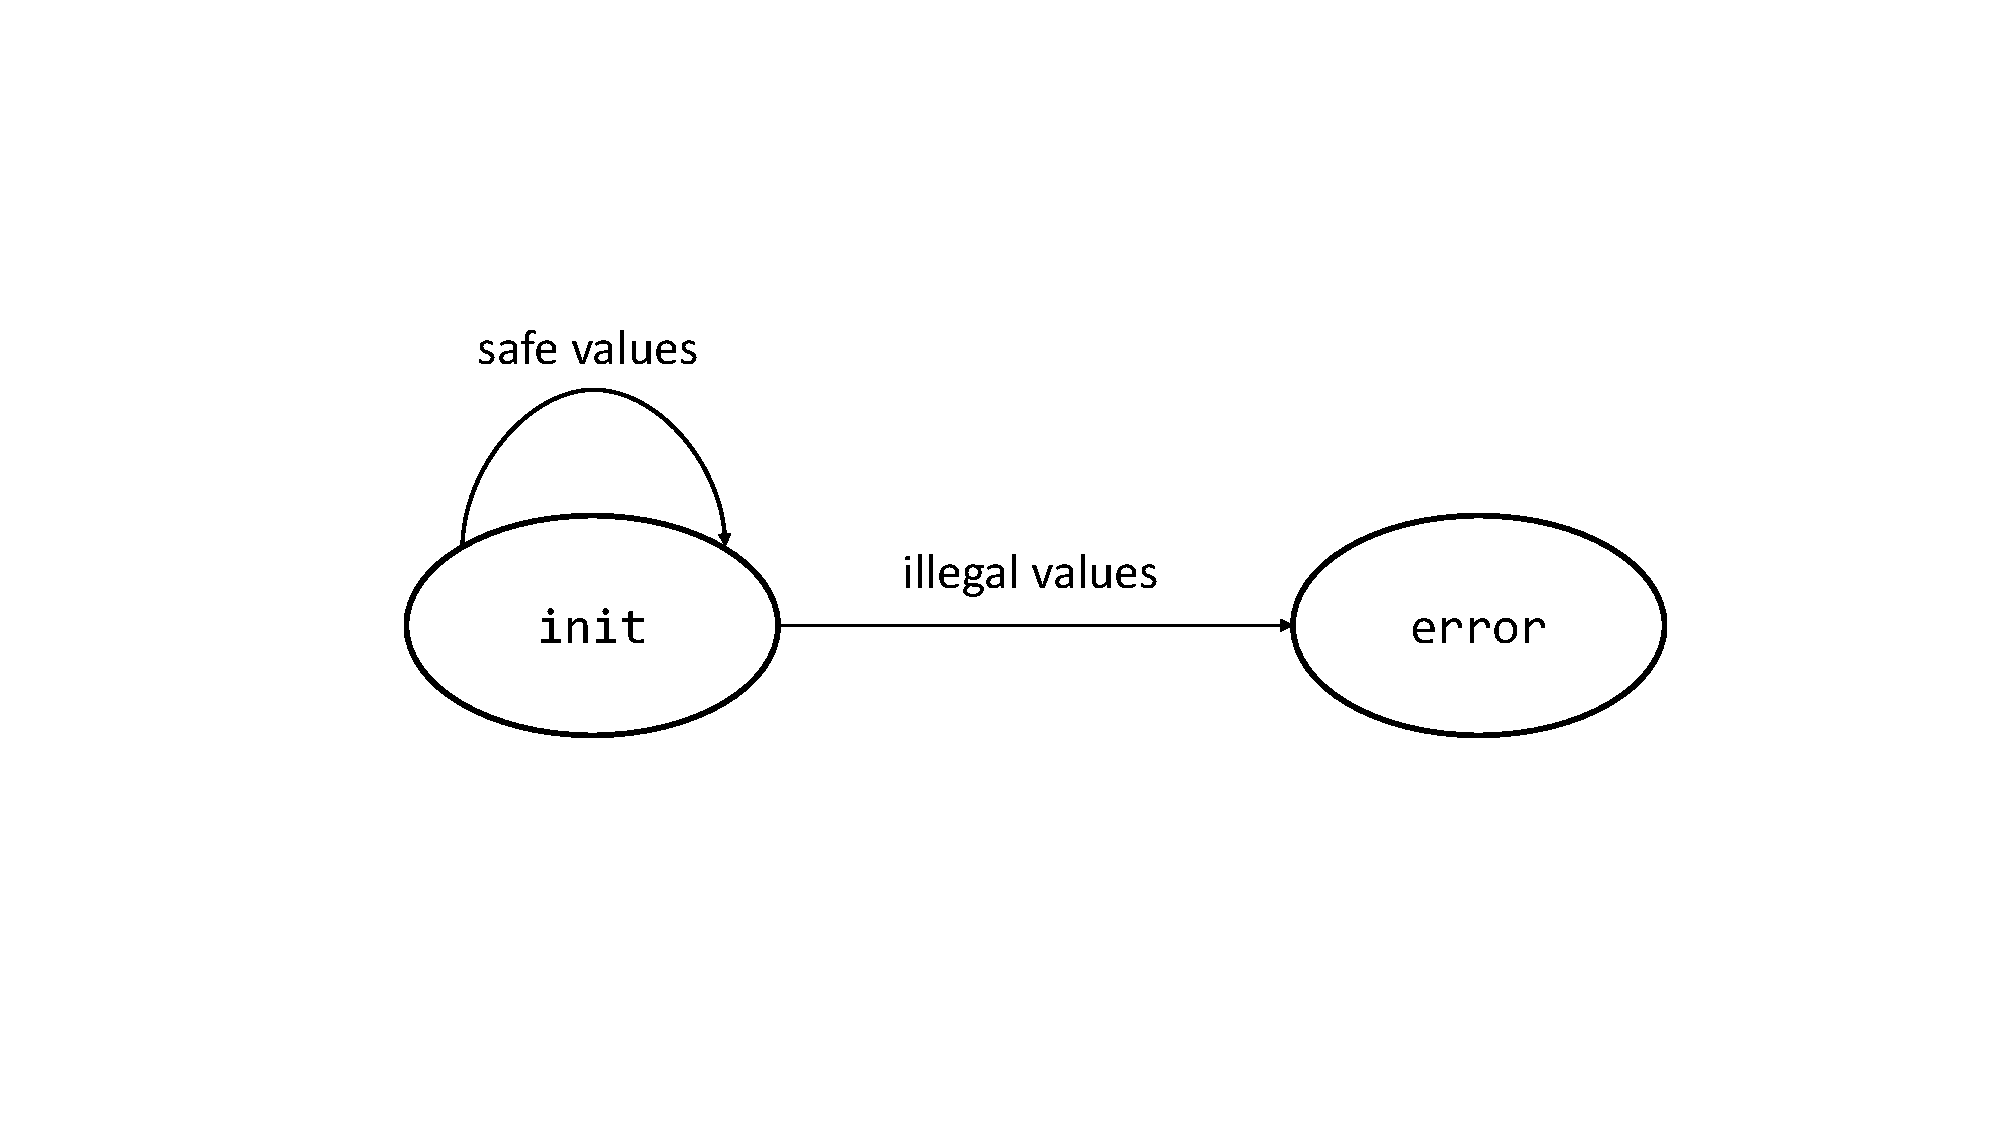
\includegraphics[width=3.2in]{images/automata.pdf}
\caption{Constraint automata general model}
\label{fig:automata}
\end{figure}

According to the Figure~\ref{fig:automata}, the repairing mechanism will only
trigger when we have a transition from 
init state to error state due to invariant violation.

\subsection{Patching Techniques}
\label{subsec:patchCA}

The patching technique is based on the exception type. 

\subsubsection{Array index out of bound exception}

Array index out of bound exception happen when one tries to access the array
with a index which is more than the size of the array or 
less than zero i.e. with some negative value. We did the patching based on these
two scenario. When the index is more than the array size, 
we patch it by assigning $array.length - 1$.

\lstset{language=Java, caption=array index out of bound patching,
label=patchingexample2}

\begin{lstlisting}[countblanklines=false]
void foo() {
    int []arr = {1,2,3,4};
    int index = 10;
    int y = 0;
    try {
	//original code
	y = arr[index];
    } catch(IndexOutOfBoundException ex) {
	//patching instrumentation
	if(index > arr.length) y = arr[arr.length - 1];
	else y = a[0];
    }
}
\end{lstlisting}

\subsubsection{Negative Array Size Exception}

Negative array size exception occurs when one tries to create a array with a
negative size. 
The patching is done based on data flow analysis. Suitable index size is
determined by looking at the successive statement dependent on the array. 
To take a safe bound, we took maximum index size and set as the array size in
the new array statement.


\lstset{language=Java, caption=arr index out of bound patching,
label=patchingexample2}

\begin{lstlisting}[countblanklines=false]
void foo() {
    int []arr = {1,2,3,4};
    int index = 10;
    int y = 0;
    try {
	//original code
	y = arr[index];
    } catch(IndexOutOfBoundException ex) {
	//patching instrumentation
	if(index > arr.length) y = arr[arr.length - 1];
	else y = a[0];
    }
}
\end{lstlisting}

\subsubsection{Arithmetic Exception : Division-by-zero Exception}

Division by zero causes arithmetic exception. There are two different cases
which were considered here. 
\begin{itemize}
 \item \textbf{Case I :} The denominator is going to the taint sink but
the left hand side is not going to any taint sink. Here we will not
manipulate the denominator as we are not manipulating any variable which are
going to any taint sink.
 \item \textbf{Case II :} The denominator and the left hand side, both are not
going to any taint sink. So they are safe to patch.
\end{itemize}

\lstset{language=Java, caption=arithmetic exception : division-by-zero patching,
label=patchingexample2}

\begin{lstlisting}[countblanklines=false]
void foo() {
    int a = 10;
    int b = 0;
    int y;
    try {
	//original code
	y = a/b;
    } catch(ArithmeticException ex) {
	//patching instrumentation
	//case I
	if(taintSink(b)) y = 0;
	//case II
	else {
	    b = 1;
	    y = a/b;
	}
    }
}
\end{lstlisting}

\subsubsection{Null Pointer Exception}

Null pointer exception in Java is the most common runtime exception
encountered. 
Thrown when an application attempts to use null in a case where an object is
required. There exists various scenarios where null pointer exception can
happen. These different scenario requires different patching techniques. Bellow
we enlist all cases and corresponding patching techniques.


\begin{itemize}
  \item \textbf{Case I} Calling the instance method of a null object. \newline
  \textbf{Patch :} This is patched by calling the constructor. In case there
  exists more than one constructor then we need to find most appropriate
  constructor. This is done by using data flow analysis in the successive
  statement to see which fields/methods been accessed and according to that
  most suitable constructor should be picked up, this will ensure safest way to
  deal with the later method calls/field accesses.
  
  \lstset{language=Java, caption=appropriate constructor,
label=patchingexample2}

\begin{lstlisting}[countblanklines=false]
class MyClass {
    Integer field1;
    String field2;
    Double field3;

    public MyClass(){
	this.field1 = 1;
	this.field2 = null;
	this.field3 = null;
    }
    public MyClass(Integer field1, String field2) {
	this.field1 = field1;
	this.field2 = field2;
	this.field3 = null;
    }
    public MyClass(Integer field1, String field2, Double field3) {
	this.field1 = field1;
	this.field2 = field2;
	this.field3 = field3;
    }
    public Double getfield3() {
	return this.field3;
    }
}

class main {
    Myclass mclass = null;
    Double a = null;
    try {
	//original code
	a = mclass.getfiled3() + 5.0;
    } catch(NullPointerException ex) {
	//instrumentation
	//choose appropriate constructor
	mlass = new MyClass(1, "a", 1.0);
	a = mclass.getfiled3();
    }
}
\end{lstlisting}
  \item 
  
  \item \textbf{Case II} Possible Accessing or modifying the field of a null
  object.\newline
  \textbf{Patch :} The patch is same as the previous one.
  
  \item \textbf{Case III} Taking the length of null as if it were an
  array.\newline
  \textbf{Patch :}The patch for this situation is very much similar to the
  negative array size exception. Here we will do a data-flow analysis to see all
  the successive statements where the array object has been used (read or
  write). For safety we will take the maximum index from those statements and
  reinitialize the array object with the size.
    
  \lstset{language=Java, caption=array null pointer exception,
  label=patchingexample2}

\begin{lstlisting}
int[] bar(int a) {
    int []arr = new int[a];
    int []b = (a > 10) ? arr:null;
    return b;
}
void foo() {
    int[] arr;
    int []arr = bar(5);
    try {
	//access or modify any field of arr
	//this will throw a null pointer exception
    } catch {
	//instrumented code
	int ARRAY_SIZE = 11;
	int []arr = new int[ARRAY_SIZE];
	//access or modify any field of arr
    }
}
\end{lstlisting}

  \item \textbf{Case IV} Accessing or modifying the slots of null as if it were
  an array.
 \textbf{Patch :} The patching mechanism is exactly same as before.
 
  \item \textbf{Case V} Throwing null as if it were a Throwable value.
\end{itemize}